\chapter{Discussion}
Please tell more about conclusion and how to the next work of this study.

\section{Aip Suprapto Munari/1164063}
\subsection{Teori}
\begin{enumerate}
\item Mengapa file suara harus dilakukan MFCC, dilengkapi dengan ilustrasi atau gambar.

Mel Frequency Cepstral Coefficients (MFCC) merupakan koefisien yang merepresentasikan audio. Sehingga diharuskannya melakukan MFCC kepada objek suara atau audio agar suara dapat berubah atau diubah ke dalam bentuk data matrix dimana telah dilakukan ekstraksi oleh MFCC kemudian direalisasikan sebagai data matrix.

\begin{itemize}
\item Ilustrasi Gambar:

\begin{figure}[ht]
\centering
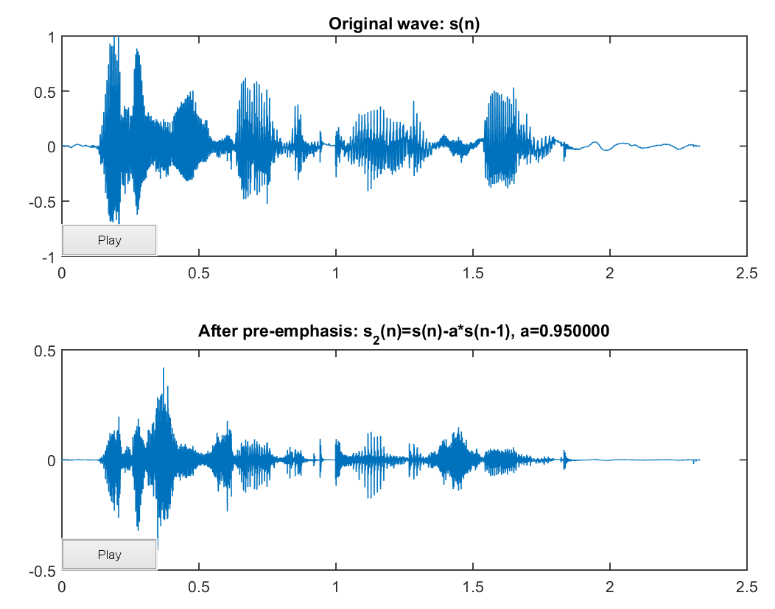
\includegraphics[scale=0.7]{figures/AIP/f1.PNG}
\caption{MFCC - Aip}
\label{MFCC - Aip}
\end{figure}

\end{itemize}

\item Konsep dasar Neural Network, dilengkapi dengan ilustrasi atau gambar.

Neural Network merupakan replika dari sistem syaraf yang terdapat pada sistem otak manusia. Dalam proses kerjanya, otak manusia disusun atas miliaran neuron dimana setiap neuron akan terhubung pada puluhan ribu neuron lain.
\begin{itemize}
\item Ilustrasi Gambar:

\begin{figure}[ht]
\centering
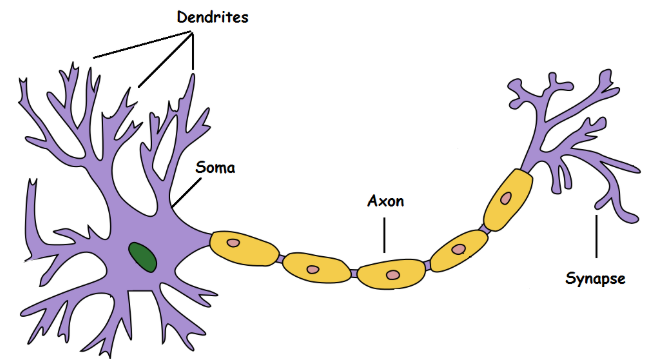
\includegraphics[scale=0.7]{figures/AIP/f2.PNG}
\caption{Konsep Dasar Neural Network - Aip}
\label{Konsep Dasar Neural Network - Aip}
\end{figure}

\end{itemize}

\item Konsep pembobotan Neural Network, dilengkapi dengan ilustrasi atau gambar.

Bobot merupakan suatu nilai yang mendefinisikan tingkat atau kepentingan hubungan antara suatu node dengan node yang lain. Semakin besar bobot suatu hubungan menandakan semakin pentingnya hubungan kedua node tersebut. Bobot merupakan suatu hubungan berupa bilangan real maupun integer, tergantung dari jenis permasalahan dan model yang digunakan. Bobot-bobot tersebut bisa ditentukan untuk berada didalam interval tertentu. selama proses pelatihan, bobot tersebut dapat menyesuaikan dengan pola-pola input.

\begin{itemize}
\item Ilustrasi Gambar :

\begin{figure}[ht]
\centering
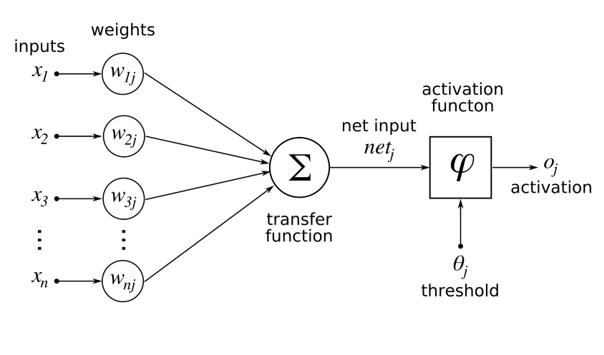
\includegraphics[scale=0.7]{figures/AIP/f3.PNG}
\caption{Konsep Pembobotan Neural Network - Aip}
\label{Konsep Pembobotan Neural Network - Aip}
\end{figure}

\end{itemize}

\item Konsep fungsi aktifasi dalam Neural Network, dilengkapi dengan ilustrasi atau gambar.
Operasi matematik yang dikenakan pada sinyal output y. Sehingga fungsi ini akan digunakan untuk pengaktifan dan juga penonaktifan neuron.
\begin{itemize}
\item Dalam konsep fungsi aktivasi Neuron Network terdapat beberapa jenis:
\begin{itemize}
\item Fungsi Undak Biner Hard Limit ( Menkonversi nilai masukan dari suatu variabel )
\item Fungsi Undak Biner Threshold ( Menggunakan nilai ambang 0 sebagai batas eksekusil )
\item Fungsi Bipolar Symetric Hard Limit ( Mempunyai keluaran bernilai 1 dan 0 )
\item Fungsi Bipolar Threshold ( Mempunyai keluaran bernilai 1, 0 atau -1 )

\item Ilustrasi Gambar:

\begin{figure}[ht]
\centering
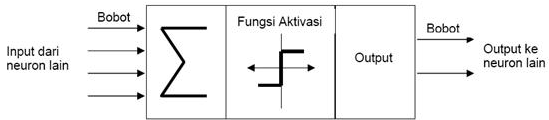
\includegraphics[scale=0.7]{figures/AIP/f4.PNG}
\caption{Konsep Fungsi Aktifasi - Aip}
\label{Konsep Fungsi Aktivasi - Aip}
\end{figure}

\end{itemize}
\end{itemize}

\item Cara membaca hasil plot dari MFCC, dilengkapi dengan ilustrasi atau gambar.

Penjelasan Cara Membaca Hasil Plot Dari MFCC :
\begin{itemize}
\item Ilustrasi Gambar :
\begin{figure}[ht]
\centering
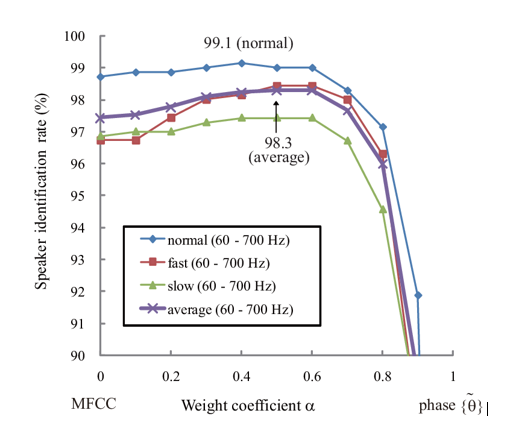
\includegraphics[scale=0.4]{figures/AIP/f5.PNG}
\caption{Plot MFCC - Aip}
\label{Plot MFCC - Aip}
\end{figure}

\end{itemize}

\item Apa itu One-Hot Encoding, dilengkapi dengan ilustrasi atau gambar.


One-Hot Encoding adalah sekelompok bit yang kombinasi hukumnya hanya terdiri dari bit dengan bit tinggi (1) dan bit lainnya rendah (0). Implementasi serupa di mana semua bit '1' kecuali satu '0' kadang-kadang disebut one-cold. Dalam statistik, variabel dummy mewakili teknik serupa untuk mewakili data kategorikal.
\begin{itemize}
\item Ilustrasi Gambar:

\begin{figure}[ht]
\centering
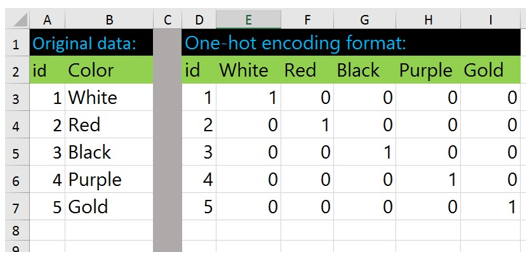
\includegraphics[scale=0.4]{figures/AIP/f6.PNG}
\caption{One-Hot Encoding - Aip}
\label{One-Hot Encoding - Aip}
\end{figure}

\end{itemize}

\item Fungsi dari np.unique dan to.categorical, dilengkapi dengan ilustrasi atau gambar.
\begin{enumerate}
\item np.unique:

Berfungsi untuk menemukan elemen unik array. Ada tiga output opsional selain elemen unik:

\begin{itemize}
\item Indeks array input yang memberikan nilai unik
\item Indeks array unik yang merekonstruksi array input
\item Berapa kali setiap nilai unik muncul dalam array input
\end{itemize}

\item Ilustrasi Gambar :

\begin{figure}[ht]
\centering
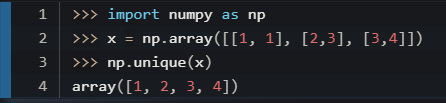
\includegraphics[scale=0.7]{figures/AIP/f7.PNG}
\caption{np.unique - Aip}
\label{np.unique - Aip}
\end{figure}

\item to.categorical:

Berfungsi untuk mengubah vektor kelas yang berupa integer menjadi matriks kelas biner.

\begin{itemize}
\item Ilustrasi Gambar :

\begin{figure}[ht]
\centering
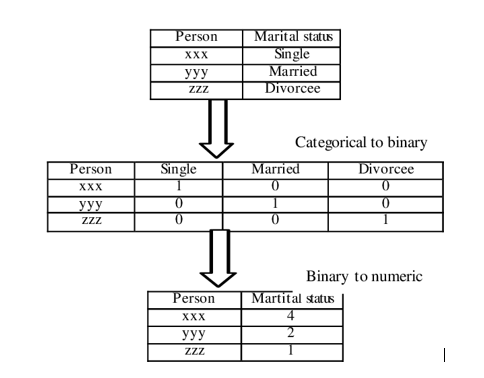
\includegraphics[scale=0.7]{figures/AIP/f7-2.png}
\caption{to.categorical - Aip}
\label{to.categorical - Aip}
\end{figure}

\end{itemize}
\end{enumerate}

\item Fungsi dari Sequential, dilengkapi dengan ilustrasi atau gambar.
Sebuah jenis model yang digunakan dalam perhitungan ataupun code program yang direalisasikan.
\begin{itemize}
\item Ilustrasi Gambar:

\begin{figure}[ht]
\centering
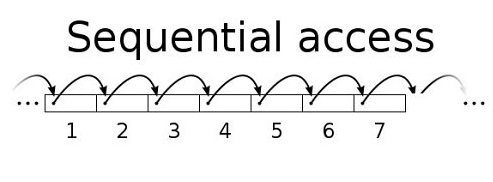
\includegraphics[scale=0.7]{figures/AIP/f8.PNG}
\caption{Sequential - Aip}
\label{Sequential - Aip}
\end{figure}

\end{itemize}
\end{enumerate}




\section{Andi Muh Aslam}
\subsection{Teori}
\begin{enumerate}
\item Kenapa File Suara Harus Dilakukan MFCC
\begin{itemize}
\item Penjelasan: Agar bisa mengubah suara menjadi vektor. Sehingga data suara bisa diolah menjadi outputan. Jadi semua parameter inputan baik itu suara, dokumen harus dipersiapkan datanya terlebih dahulu, kalau untuk dokumen untuk teks menggunakan word2vec, sedangkan untuk suara menggunakan MFCC (Mel Frequency Cepstral Coeficients) 

\item Ilustrasi Gambar
\begin{figure}[!hbtp]
\centering
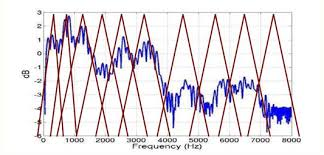
\includegraphics[scale=0.7]{figures/andi/61.jpg}
\caption{MFCC}
\label{Contoh 1}
\end{figure}
\end{itemize}


\item Konsep Dasar Neural Network
\begin{itemize}
\item  Penjelasan:
\par Neural Network merupakan sistem komputasi yang efisien dimana tema utamanya dipinjam dari analogi jaringan saraf biologis. Neural Network biasa disebut dengan jaringan saraf tiruan dimana Neural Network sebenarnya mengadopsi dari kemampuan otak manusia yang mampu memberikan stimulasi/rangsangan, melakukan proses, dan memberikan output.

\item Ilustrasi Gambar
\begin{figure}[!hbtp]
\centering
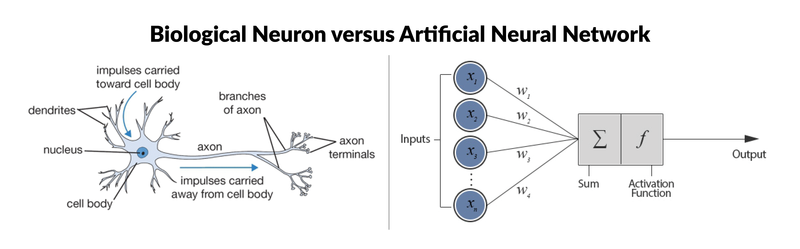
\includegraphics[scale=0.3]{figures/andi/62.png}
\caption{Konsep Dasar Neural Network}
\label{Contoh 2}
\end{figure}

\end{itemize}

\item Konsep Pembobotan Dalam Neural Network
\begin{itemize}
\item Penjelasan:
\par Cara kerja Neural Network dapat dianalogikan sebagaimana halnya manusia belajar dengan mengunakan contoh atau yang disebut sebagai supervised learning. Sebuah Neural Network dikonfigurasi untuk aplikasi tertentu, seperti pengenalan pola atau klasifikasi data, dan kemudian disempurnakan melalui proses pembelajaran. Proses belajar yang terjadi dalam sistem biologis melibatkan penyesuaian koneksi sinaptik yang ada antara neuron, dalam halnya pada Neural Network penyesuaian koneksi sinaptik antar neuron dilakukan dengan menyesuaikan nilai bobot yang ada pada tiap konektivitas baik dari input, neuron maupun output.

\item Ilustrasi Gambar
\begin{figure}[!hbtp]
\centering
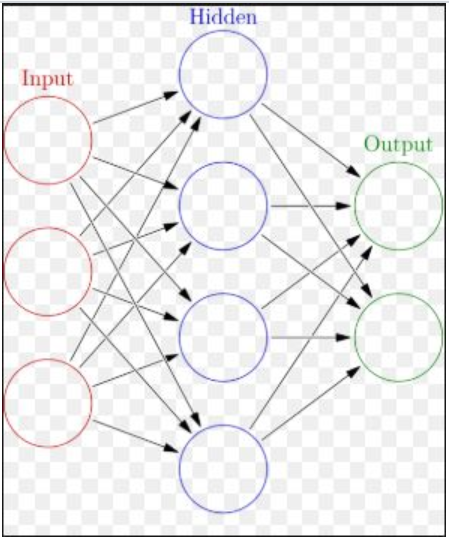
\includegraphics[scale=0.3]{figures/andi/63.PNG}
\caption{Konsep Pembobotan}
\label{Contoh 3}
\end{figure}

\end{itemize}


\item Konsep Fungsi Aktivasi Dalam Neural Network
\begin{itemize}
\item Penjelasan:
\par Setiap neuron mempunyai tingkat aktivasi yang merupakan fungsi dari input yang masuk padanya. Aktivasi yang dikirim suatu neuron ke neuron lain berupa sinyal dan hanya dapat mengirim sekali dalam satu waktu, meskipun sinyal tersebut disebarkan pada beberapa neuron yang lain.

\item Ilustrasi Gambar
\begin{figure}[!hbtp]
\centering
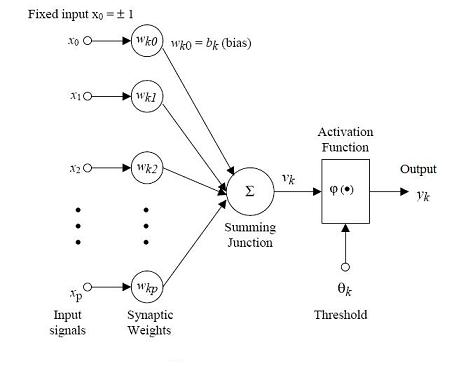
\includegraphics[scale=0.7]{figures/andi/64.jpg}
\caption{Konsep Aktivasi}
\label{Contoh 4}
\end{figure}

\end{itemize}


\item Cara Membaca Hasil Plot Dari MFCC
\begin{itemize}
\item Penjelasan:
\par Cara membaca hasil plot dari MFCC yaitu Nanti akan ada outputan berbentuk grafik setelah melakukan plot dari MFCC. Kemudian terdapat frekuensi/Hz pada suara frekuensi biasanya vertikal atau biasa disimbolkan dengan sumbu y, Lalu terdapat waktu yang mana waktu diartikan dalam simbol sumbu x. Sedangkan pada bagian dalam atau bisa disimbolkan dengan sumbu z merupakan power atau kekuatan dari lagu atau suara atau desibel yang dihasilkan. Untuk warna biru itu merupakan suara rendah, yang merah merupakan tinggi apabila daya frekuensi nya misalkan suara siul berarti dominan warna merah karena siul biasanya pada nada yang tinggi sedangkan jika bass dominan biru karena bass merupakan nada rendah. 

\item Ilustrasi Gambar
\begin{figure}[!hbtp]
\centering
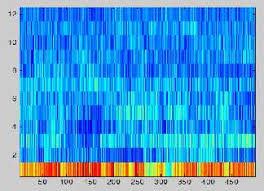
\includegraphics[scale=0.5]{figures/andi/65.jpg}
\caption{Cara Membaca Hasil Plot MLCC}
\label{Contoh 5}
\end{figure}

\end{itemize}




\item Apa Itu One-Hot Encoding?
\begin{itemize}
\item Penjelasan:
\par One-hot encoding adalah representasi dari variabel kategori sebagai vektor biner. Yaitu nilai kategorika harusl dipetakan ke nilai integer. Kemudian, setiap nilai integer direpresentasikan sebagai vektor biner yang semuanya bernilai nol kecuali indeks integer, yang ditandai dengan 1.
\item Ilustrasi Gambar
\begin{figure}[!hbtp]
\centering
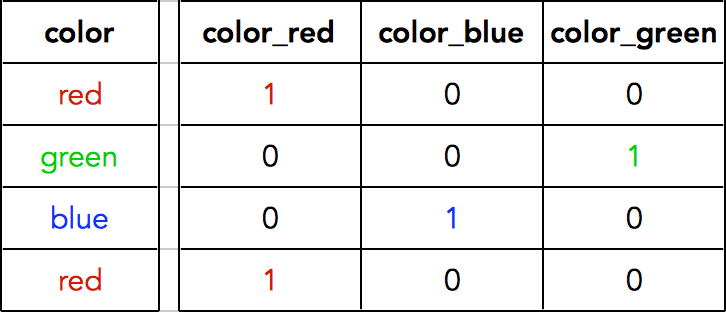
\includegraphics[scale=0.5]{figures/andi/66.png}
\caption{One Hot Encoding}
\label{Contoh 6}
\end{figure}
\end{itemize}


\item Fungsi Dari np unique dan to categorical dalam kode program
\begin{itemize}
\item  Np.unique

\item Penjelasan: np.unique untuk mengekstaksi elemen-elemen unik tertentu dalam array.
\begin{figure}[!hbtp]
\centering
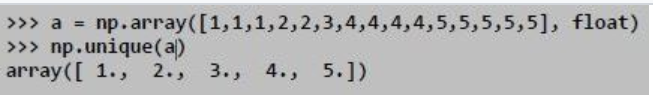
\includegraphics[scale=0.7]{figures/andi/67.png}
\caption{NP Unique}
\label{Contoh 7}
\end{figure}


\end{itemize}
\begin{itemize}
\item  To categorical
\item Penjelasan: Berfungsi untuk mengubah vektor kelas yang berupa integer ( number ) menjadi matriks kelas biner.	
\begin{figure}[!hbtp]
\centering
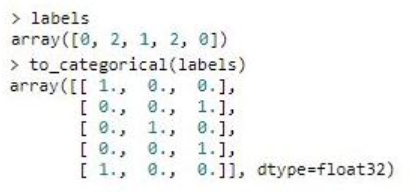
\includegraphics[scale=0.7]{figures/andi/67_1.PNG}
\caption{To Categorical}
\label{Contoh 7_1}
\end{figure}
\end{itemize}


\item Fungsi Dari Sequential Pada Kode Program
\begin{itemize}
\item Penjelasan:
\par Fungsi dari Sequential dalam kode program yaitu meruapakan sebuah jenis model yang digunakan dalam perhitungan ataupun code program yang direalisasikan. Neural Networks Sequential membangun fitur tingkat tinggi melalui lapisan yang berurutan. Sequential juga merupakan proses dimana membandingkan setiap elemen larik satu per satu secara beruntun, mulai dari elemen pertama, sampai dengan elemen terakhir atau elemen yang dicari sudah ditemukan.
\item Ilustrasi Gambar
\begin{figure}[!hbtp]
\centering
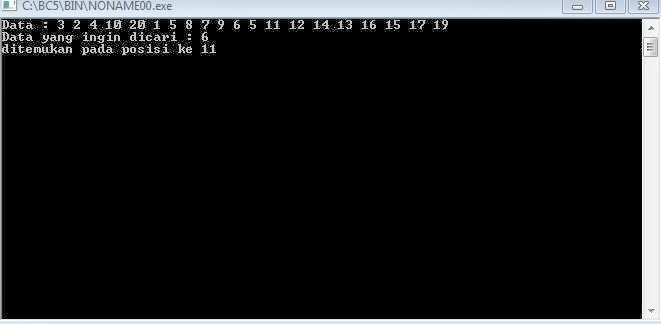
\includegraphics[scale=0.8]{figures/andi/68.jpg}
\caption{Sequential}
\label{Contoh 8}
\end{figure}
\end{itemize}

\end{enumerate}

